\section{Introduction}

With an estimated 4 billion units in use in December 2008, mobile
devices have already become the most popular computing device in human
history. Their portability and communication capabilities have
revolutionized how people interact with each other. Despite the rapid
growth of mobile phones, text entry on mobile devices remains a major
challenge. However, with the recent rise in sales in the
smartphone/PDA market and the recent launch of products like iPad,
users have greater access to medium sized touch screens. These screens
should offer more screen space than a traditional phone, and can
arguably be more effective in text-input tasks. However, due to
increased size and weight, these devices require specific postures
from the users to be able to input text.

Recently, there has been a push in the industry for devices with
backside input. Notion ink's Adam PC has a backside trackpad
[Reference]. Samsung and Toshiba have also been making effort towards
backside touch input [Reference]. With the growing interest in
backside touch input, comes the potential of using the same for
manipulating information. A "natural" method of holding such a device
is to have hands on both the sides with fingers wrapped around on the
back [Figure]. The advantage of having a backside touch input is that
users can possibly use the fingers on the back to input text and
manipulate information.

Moreover, the tablet form-factor introduces two problems for the user.
First, since a tablet is very portable, it is an ideal device for use
while mobile (e.g. actually moving, rather than nomadic, meaning in
different places, but mostly stationary).  Doctors in a busy hospital,
commuters standing on a train and TV producers on location at a shoot
are all examples of users who would benefit from using a computing
device while standing, walking or sitting and briefly holding their
device.

\begin{figure}
    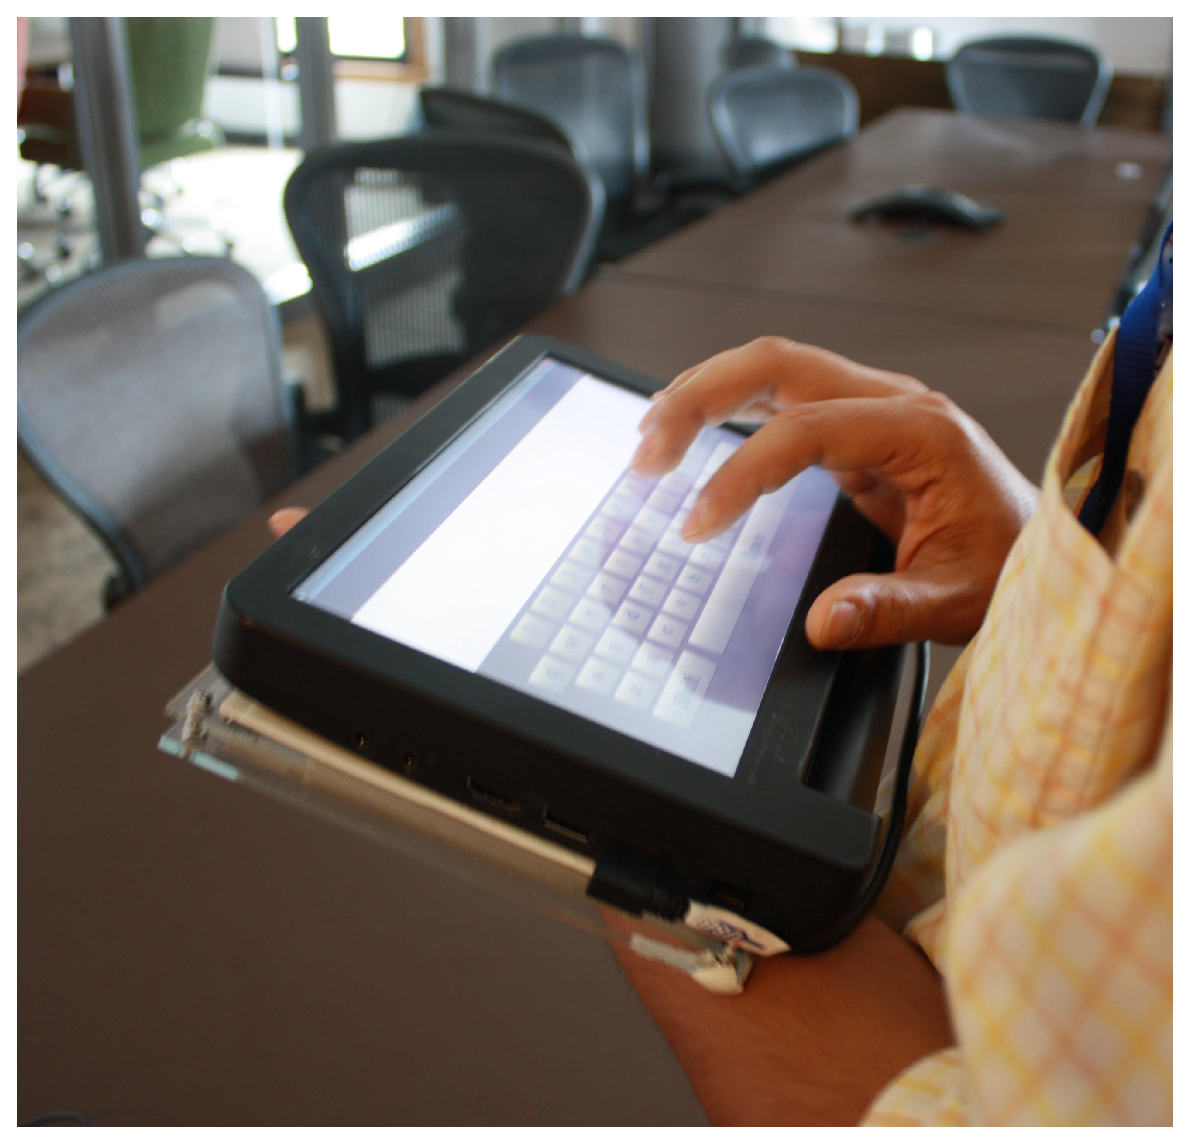
\includegraphics[scale=0.35]{Figures/device_hold.eps} 
  	\caption{A user holding a foot-scale device and trying to enter text. It can be seen how this is unstable and unnatural.}
\end{figure}

Unlike a mobile phone, however, a larger (e.g. 7+ inches wide)
keyboard (soft or otherwise) does not work well with two thumbs
because of the relatively large distance that the thumbs must travel
to reach the appropriate keys, and the weight of the device compounds
the problem of typing by straining the hands to support the device
while making precise movements to position the thumbs over the proper
keys. (drawing) While standing, many users resort to a different pose,
in which one arm supports the device while the other hand types with a
single finger.

A second difficulty, common to all soft keyboards, arises because the
fingers do not receive any tactile feedback as to their position on
the keyboard.  Unlike a physical keyboard in which the keys have
ridges that delineate their boundaries, a soft keyboard often requires
the user to look at the keyboard to ensure that they are activating
the correct keys.  Looking at the keys while typing is distracting,
requires many eye shifts (since the user must also verify on the
screen that what they are typing is correct).  This can be alleviated
to some extent by providing haptic feedback when a key is activated,
but this provides only limited improvement.

\begin{figure}
    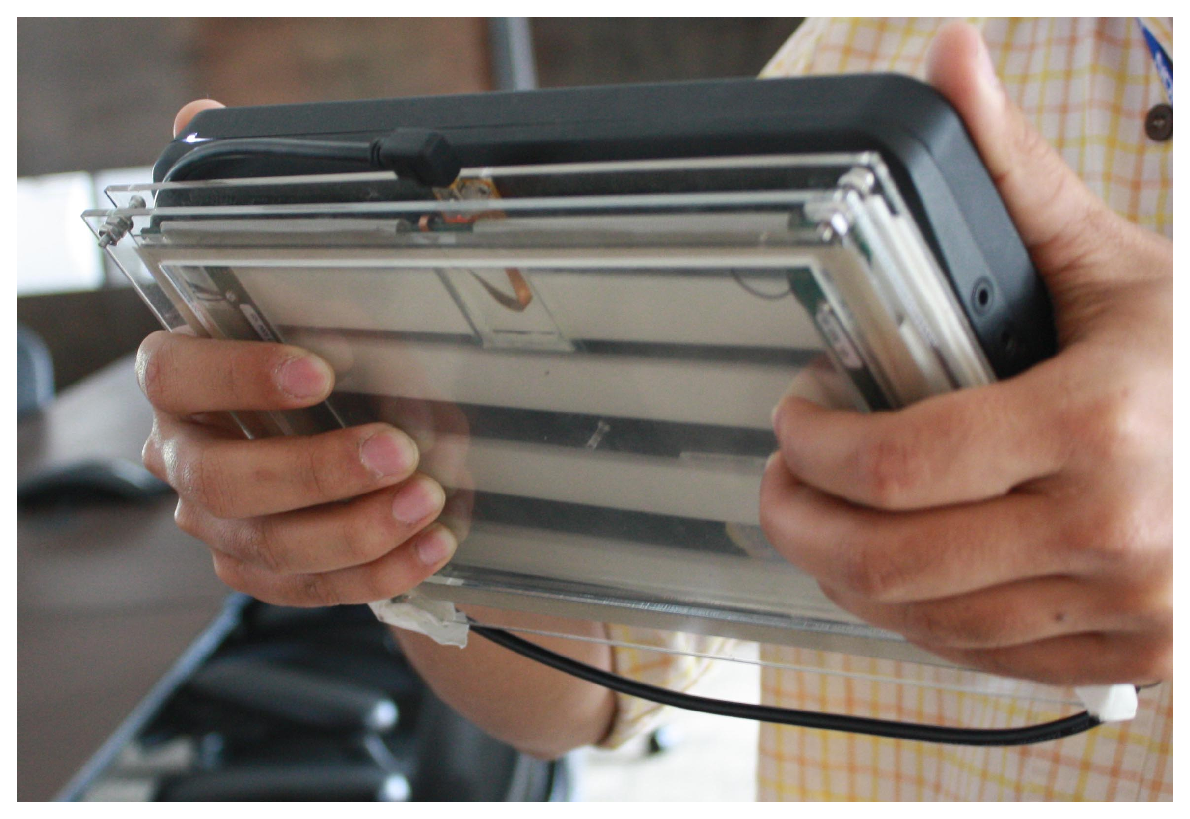
\includegraphics[scale=0.43]{Figures/natural1.eps} 
     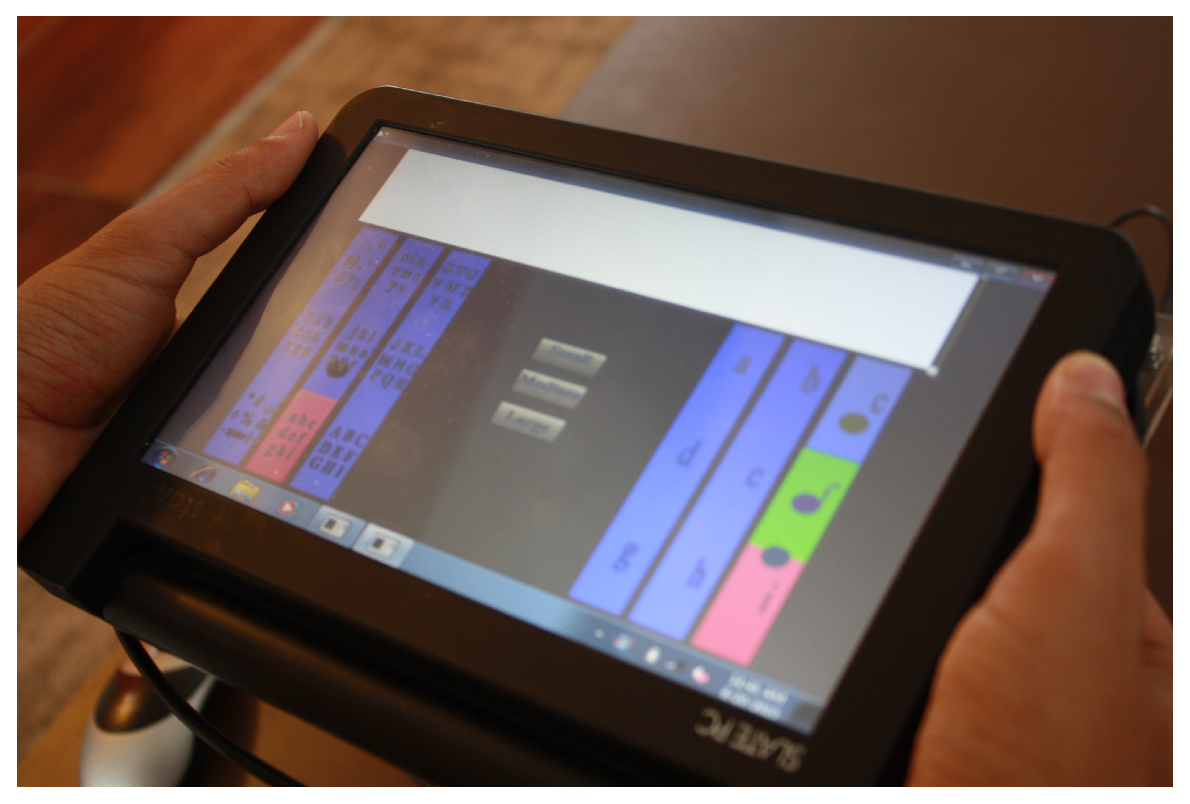
\includegraphics[scale=0.43]{Figures/natural2.eps} 
  	\caption{A user holding a foot-scale device in a natural and stable posture. The user is able to see his finger positions on the screen on the front.}
\end{figure}

In this paper we present novel methods that investigate the use of a
backside touch input device for text input on a foot-scale mobile
device. We implement two mechanisms, one of them being a backside
QWERTY keyboard, the other one being a chording mechanism. We compare
and contrast the performance of these novel mechanisms with a standard
soft QWERTY keyboard.
